\documentclass[conference]{IEEEtran}

\usepackage{cite}
\usepackage{amsmath,amssymb,amsfonts}
\usepackage{graphicx}
\usepackage{hyperref}
\usepackage{booktabs}
\usepackage{multirow}
\usepackage{makecell}
\usepackage{silence}
\WarningFilter{caption}{Unknown document class}
\usepackage{caption}
\usepackage{graphicx}

\graphicspath{ {./images/} }

\title{Impact of Secure Aggregation and Differential Privacy on 
Federated Network Intrusion Detection Systems}

\author{
\IEEEauthorblockN{Carlos Andrés Peña Arias}
\IEEEauthorblockA{
Department of Systems and Computing Engineering\\
Universidad de los Andes\\
Bogotá, Colombia\\
\textit{c.penaa@uniandes.edu.co}}
}

\begin{document}

\maketitle

\begin{abstract}
    Federated Learning (FL) facilitates the joint training of machine learning models without centralizing sensitive data, making it highly suitable for Network Intrusion Detection Systems (NIDS). However, FL is vulnerable to inference attacks that may compromise training data privacy and data exposure attacks by honest-but-curious servers \cite{ameria2023}. To mitigate these risks, privacy-preserving mechanisms such as Differential Privacy (DP) and Secure Aggregation (SecAgg) are employed \cite{khraisat2024}. This work presents an empirical evaluation of the impact of DP and SecAgg on the performance of a federated NIDS using  industry-oriented framework NVIDIA FLARE (NVFlare).
    % #TODO verify:
    % Results show that while SecAgg preserves model accuracy with increased
    % computational cost, DP introduces a measurable degradation in performance
    % proportional to the noise level. A trade-off analysis between privacy,
    % performance, and computational cost is presented.
\end{abstract}

\begin{IEEEkeywords}
    Federated Learning, Network Intrusion Detection Systems, Differential Privacy, Secure Aggregation, NVFlare, Cybersecurity
\end{IEEEkeywords}

\section{Introduction}

Modern NIDS rely more and more on machine learning (ML) and deep learning (DL), which require access to large datasets to efficiently and accurately identify cyber threats \cite{khraisat2024}. 

Traditional centralized approaches introduce privacy risks and regulatory challenges due to data concentration and storage of sensitive information. FL addresses these issues by enabling distributed model training without sharing raw data \cite{yurdem2024}. However, FL remains vulnerable to inference attacks, including membership inference, which can expose whether specific samples were used during training \cite{ameria2023}. Additionally, FL is vulnerable to data exposure attacks and data poisoning attacks by honest-but-curious servers \cite{he2025}.

To mitigate these risks, additional privacy-preserving mechanisms such as DP and SecAgg are integrated into FL pipelines \cite{khraisat2024}. DP protects individual data points by injecting controlled noise, while SecAgg ensures that the server only observes aggregated model updates.

This paper evaluates the impact of these mechanisms on model performance, privacy, and computational cost in a realistic federated NIDS setting using industry-oriented framework NVFlare.

\section{Related Work}

Federated Learning has gained significant attention in domains such as critical infrastructure, healthcare, and finance due to its privacy-preserving capabilities \cite{yurdem2024}. In the context of NIDS, FL enables collaborative training across distributed environments without exposing sensitive data.

Despite these advantages, FL introduces several challenges, including vulnerability to inference attacks, communication overhead, and data heterogeneity \cite{khraisat2024}. In particular, inference attacks pose a major risk, as adversaries can extract sensitive information from model updates \cite{ameria2023}.

Recent work has explored privacy-preserving FL for intrusion detection, but often lacks comprehensive experimental evaluation using large-scale datasets and  industry-oriented frameworks (that integrate DP and SecAgg to address prior mentioned challenges) \cite{torre2024}. Additionally, there is limited analysis of the quantitative trade-off between privacy, performance and computational cost in this context.

\section{Methodology}

\subsection{Research Methodology}

This study follows a quantitative experimental research methodology to evaluate the impact of privacy-preserving mechanisms in FL-NIDS. Experimental research is a methodology in which controlled variables are systematically manipulated to measure their effect on specific outcomes. In ML and cybersecurity research, this methodology is commonly used to evaluate how architectural or algorithmic modifications influence model behavior, performance, and computational efficiency.

This methodology was selected because the objective of this work is to analyze the trade-offs introduced by SecAgg and DP in a FL environment. Specifically, the study aims to determine how these privacy-preserving mechanisms affect intrusion detection performance, privacy guarantees, and computational cost under controlled experimental conditions.

The experimental process was structured in multiple stages. First, a centralized baseline was established using the GraphIDS architecture trained on the NF-CSE-CIC-IDS2018-v3 dataset. Second, the same model was adapted to a federated learning environment using NVFlare while maintaining consistent hyperparameters and training configurations to ensure a fair comparison. Third, DP and SecAgg mechanisms were integrated (separately) into the federated pipeline. Finally, the resulting configurations were evaluated and compared using performance metrics, privacy measurements, and computational cost indicators.

The independent variables considered in this study are: learning architecture (centralized or federated), use of privacy-preserving mechanism (SecAgg or DP), and noise multiplier. The dependent variables are: Macro F1-score, Precision-Recall Area Under the Curve (PR-AUC), training time, and communication overhead.

All experiments were conducted under the same hardware and software conditions to improve reproducibility and ensure consistency between evaluations.

\subsection{Research Questions}

To evaluate the impact of privacy-preserving mechanisms on FL-NIDS, the research is guided by the following questions:

RQ1: How does the performance of a federated GraphIDS model compare to its centralized counterpart in terms of intrusion detection capability?

RQ2: What impact does SecAgg have on the computational cost and performance of FL-NIDS?

RQ3: How does DP affect the trade-off between privacy guarantees and model performance of FL-NIDS?

\subsection{Experimental Environment}

All experiments were conducted on a single workstation equipped with an NVIDIA RTX 4090 GPU with 24GB of VRAM, an AMD Ryzen 7 5800X3D CPU, and 32GB of RAM. This configuration provides sufficient computational resources for training graph-based deep learning models while remaining representative of accessible high-end consumer hardware rather than enterprise-grade infrastructure.

The FL pipeline was implemented using the NVFlare framework. The experiments were executed within a Windows Subsystem for Linux (WSL) environment, where multiple client processes and the federated server were simulated on the same physical machine using NVFlare's Proof-of-Concept (POC) deployment mode.

To ensure consistency and reproducibility across experiments, the same codebase, model architecture, preprocessing pipeline, and training hyperparameters were maintained for both centralized and federated configurations. This approach minimizes implementation variability and enables a fair comparison between the evaluated privacy-preserving mechanisms.

The implementation developed for this work is publicly available in the following repository: \url{https://github.com/carandp/FL-NIDS}.

\subsection{Dataset and Sampling Strategy}
\label{subsec:dataset_sampling}

The experiments were conducted using the NF-CSE-CIC-IDS2018-v3 dataset, a NetFlow-based intrusion detection dataset derived from the CSE-CIC-IDS2018 traffic collection environment \cite{luay2026}. The original dataset was generated from a large-scale AWS-based infrastructure containing multiple departments, servers, and attacker machines, providing realistic network traffic for intrusion detection research \cite{csecicids2018}. 

The dataset was selected due to its suitability for modern ML-based NIDS, its large-scale traffic diversity, and its compatibility with graph-based intrusion detection approaches such as GraphIDS.

Due to hardware and training-time constraints, a representative subset of the dataset was constructed for experimentation. The sampling strategy was designed to preserve realistic traffic distributions while reducing dataset size to a manageable scale for repeated federated experiments.

Network flows were grouped according to their associated ports and services into three traffic categories:

\begin{itemize}
    \item Web Services
    \item File Server and Remote Services
    \item Database Services
\end{itemize}

The resulting category distribution is shown in \autoref{tab:port_stats}.

\begin{table}[ht]
    \centering
    \renewcommand{\arraystretch}{1.3}
    \begin{tabular}{|l|l|l|l|}
        \hline
        \textbf{Category} & \textbf{Port} & \textbf{Flows} & \textbf{Distribution} \\ \hline
        \multirow{2}{*}{Web} & 80 (HTTP) & \multirow{2}{*}{3,081,661} & \textbf{Benign:} 43.81\% \\ \cline{2-2}
         & 8080 (HTTP) & & \textbf{Malicious:} 56.19\% \\ \hline
        \multirow{6}{*}{\begin{tabular}[l]{@{}l@{}}File Server and\\ Remote\end{tabular}} & 21 (FTP) & \multirow{6}{*}{5,578,635} & \multirow{6}{*}{\begin{tabular}[c]{@{}l@{}}\textbf{Benign:} 87.46\%\\ \textbf{Malicious:} 12.54\%\end{tabular}} \\ \cline{2-2}
         & 22 (SFTP) & & \\ \cline{2-2}
         & 138 (NetBIOS) & & \\ \cline{2-2}
         & 139 (NetBIOS) & & \\ \cline{2-2}
         & 445 (SMB) & & \\ \cline{2-2}
         & 3389 (RDP) & & \\ \hline
        \multirow{2}{*}{Database} & 1433 (MSSQL) & \multirow{2}{*}{10,967} & \textbf{Benign:} 97.46\% \\ \cline{2-2}
         & 3306 (MySQL) & & \textbf{Malicious:} 2.54\% \\ \hline
    \end{tabular}
    \caption{Port Categories and Flow Distributions}
    \label{tab:port_stats}
\end{table}

For the Web and File Server and Remote categories, samples were sorted according to flow start time, and the first 25\% of the observations were selected. Temporal sampling was preferred over random sampling to preserve chronological traffic behavior and maintain realistic sequential flow distributions. This approach preserves temporal consistency while reducing dataset size for training and evaluation.

The final sampled dataset composition is presented in \autoref{tab:final_subdataset}. The resulting subset maintains representative traffic diversity while improving computational feasibility for repeated centralized and federated training experiments.


\begin{table}[ht]
    \centering
    \renewcommand{\arraystretch}{1.3}
    \begin{tabular}{|l|l|l|l|}
        \hline
        \textbf{Category} & \textbf{Port} & \textbf{Flows} & \textbf{Distribution} \\ \hline

        % Web Group
        \multirow{2}{*}{Web} & 80 (HTTP) & \multirow{2}{*}{770,415} & \textbf{Benign:} 43.81\% \\ \cline{2-2}
         & 8080 (HTTP) & & \textbf{Malicious:} 56.19\% \\ \hline

        % File Server and Remote Group
        \multirow{6}{*}{\begin{tabular}[l]{@{}l@{}}File Server and\\ Remote\end{tabular}} & 21 (FTP) & \multirow{6}{*}{1,394,658} & \multirow{6}{*}{\begin{tabular}[c]{@{}l@{}}\textbf{Benign:} 87.46\%\\ \textbf{Malicious:} 12.54\%\end{tabular}} \\ \cline{2-2}
         & 22 (SFTP) & & \\ \cline{2-2}
         & 138 (NetBIOS) & & \\ \cline{2-2}
         & 139 (NetBIOS) & & \\ \cline{2-2}
         & 445 (SMB) & & \\ \cline{2-2}
         & 3389 (RDP) & & \\ \hline

        % Database Group
        \multirow{2}{*}{Database} & 1433 (MSSQL) & \multirow{2}{*}{10,960} & \textbf{Benign:} 97.52\% \\ \cline{2-2}
         & 3306 (MySQL) & & \textbf{Malicious:} 2.48\% \\ \hline
    \end{tabular}
    \caption{Final Sampled Subdataset Composition}
    \label{tab:final_subdataset}
\end{table}

The dataset partitioning strategy was also aligned with the federated learning setup. Each client received a distinct traffic category to simulate heterogeneous network environments commonly found in real-world distributed infrastructures. The client distribution is summarized in \autoref{tab:client_mapping}.

\begin{table}[ht]
    \centering
    \renewcommand{\arraystretch}{1.3}
    \begin{tabular}{|l|l|}
        \hline
        \textbf{Client ID} & \textbf{Data Subsample} \\ \hline
        client0 & Web \\ \hline
        client1 & File Server and Remote \\ \hline
        client2 & Database \\ \hline
    \end{tabular}
    \caption{Mapping of Client IDs to Network Traffic Subsamples}
    \label{tab:client_mapping}
\end{table}

\subsection{Centralized Baseline}

To establish a reference point for subsequent federated learning experiments, a centralized baseline was implemented using the GraphIDS architecture proposed by Guerra et al. \cite{guerra2025}. GraphIDS is a self-supervised graph-based intrusion detection model designed to learn network behavior representations directly from communication patterns without requiring fully labeled attack data.

The model combines Graph Neural Networks (GNNs) with a Transformer-based masked autoencoder architecture to capture both local structural relationships and global traffic patterns within network flow graphs. This design makes GraphIDS particularly suitable for intrusion detection tasks involving complex communication dependencies and heterogeneous traffic behavior.

GraphIDS was selected for this study due to its competitive performance in intrusion detection tasks, compatibility with graph-structured network traffic data, and suitability for adaptation into federated learning environments.

The centralized model was trained using the sampled NF-CSE-CIC-IDS2018-v3 subset described in the previous section. The training configuration and preprocessing pipeline were maintained consistently across all subsequent federated experiments to ensure fair comparison between centralized and distributed learning scenarios.

The centralized baseline was evaluated using the following metrics: Macro F1-score, PR-AUC, and Training time.

These metrics were selected to evaluate classification effectiveness under class imbalance conditions while also measuring computational cost during training.

\subsection{Federated Learning Setup}
\label{subsec:federated_learning_setup}

The centralized GraphIDS model was adapted into a FL environment using the industry-oriented NVFlare framework \cite{roth2024}. The federated setup simulates distributed network environments in which multiple clients collaboratively train a shared global model without exchanging raw network traffic data.

To emulate realistic heterogeneous network conditions, the dataset was partitioned according to the traffic categories described previously. Each client received a distinct subset of network traffic corresponding to different services and infrastructure roles. This configuration introduces non-identically distributed (non-IID) data across clients, reflecting realistic federated intrusion detection scenarios where organizations may observe different traffic behaviors and attack distributions.

Federated training was performed using the Federated Averaging (FedAvg) aggregation algorithm. FedAvg was selected due to its widespread adoption as a baseline aggregation strategy in federated learning research and its compatibility with heterogeneous client environments. During training, each client performs local model updates using its private dataset, after which the server aggregates the resulting model parameters to produce an updated global model.

One of the main challenges observed in the federated setting was severe class imbalance across certain client datasets, particularly in the Database traffic category, where malicious samples represented only a small fraction of the available flows. In highly imbalanced intrusion detection scenarios, federated clients may fail to adequately learn minority attack patterns, negatively affecting the global model’s detection capability.

To mitigate this issue, local oversampling was applied during client-side training using the BorderlineSMOTE technique. BorderlineSMOTE was selected because it focuses synthetic sample generation near decision boundaries, where minority malicious samples are more difficult to classify. This approach was used only when the minority class ratio fell below a threshold of 5\%, helping improve malicious representation while avoiding unnecessary oversampling in more balanced client datasets.

The federated training pipeline maintained the same model architecture, preprocessing pipeline, and training hyperparameters used in the centralized baseline to ensure fair comparison between centralized and federated configurations. The FL hyperparameters can be seen in \autoref{tab:fed_hyperparameters}.

\begin{table}[h]
    \centering
    \renewcommand{\arraystretch}{1.3}
    \begin{tabular}{|l|c|}
        \hline
        \textbf{Parameter} & \textbf{Value} \\ \hline
        Aggregation Algorithm & FedAvg \\ \hline
        Number of Clients & 3 \\ \hline
        Local Epochs & 2 \\ \hline
        Communication Rounds & 100 \\ \hline
    \end{tabular}
    \caption{Federated Learning Hyperparameters}
    \label{tab:fed_hyperparameters}
\end{table}

For each experimental configuration, the global model was evaluated after federated aggregation rounds using the same performance metrics defined for the centralized baseline. Additionally, communication overhead metric was collected to evaluate the computational impact introduced by distributed training and privacy-preserving mechanisms.

The federated environment was executed using NVFlare’s Proof-of-Concept (POC) deployment mode, where multiple clients, the federated server, and the administration console were simulated as independent processes on a single physical machine \cite{nvflare_poc_doc}.

\subsection{Secure Aggregation}
\label{subsec:secure_aggregation}

To protect client model updates during federated training, a SecAgg mechanism based on Homomorphic Encryption (HE) was integrated into the FL pipeline using the TenSEAL library and NVFlare's built-in SecAgg components.

The implementation uses the CKKS (Cheon-Kim-Kim-Song) HE scheme, which supports approximate arithmetic operations over encrypted floating-point vectors \cite{cheon2017}. CKKS was selected due to its suitability for machine learning workloads, where model parameters are represented as real-valued tensors and efficient encrypted aggregation is required.

The SecAgg environment was configured using NVFlare's cryptographic builders, including: certificate generation for secure client-server communication, digital signature support for update integrity verification, and HE context generation for encrypted model aggregation.

The HE configuration used in this work includes:

\begin{itemize}
    \item Polynomial modulus degree: 8192
    \item Coefficient modulus bit sizes: [60, 40, 40]
    \item Scaling factor bits: 40
    \item Encryption scheme: CKKS
\end{itemize}

During federated training, client model updates are encrypted locally before transmission to the aggregation server. As a result, the server never accesses plaintext client weights or gradients. Instead, the server performs FedAvg directly over encrypted model parameters and returns the aggregated encrypted global model to the clients for decryption and subsequent training rounds.

This approach reduces the risk of sensitive information leakage from individual client updates while preserving the collaborative training process required in federated learning environments.

\subsection{Differential Privacy}

To mitigate inference attacks against client model updates, DP was integrated into the FL pipeline through a client-side Gaussian perturbation mechanism applied before model updates were transmitted to the aggregation server as shown in \autoref{fig:dp_pipeline}.

\begin{figure}[h]
    \centering
    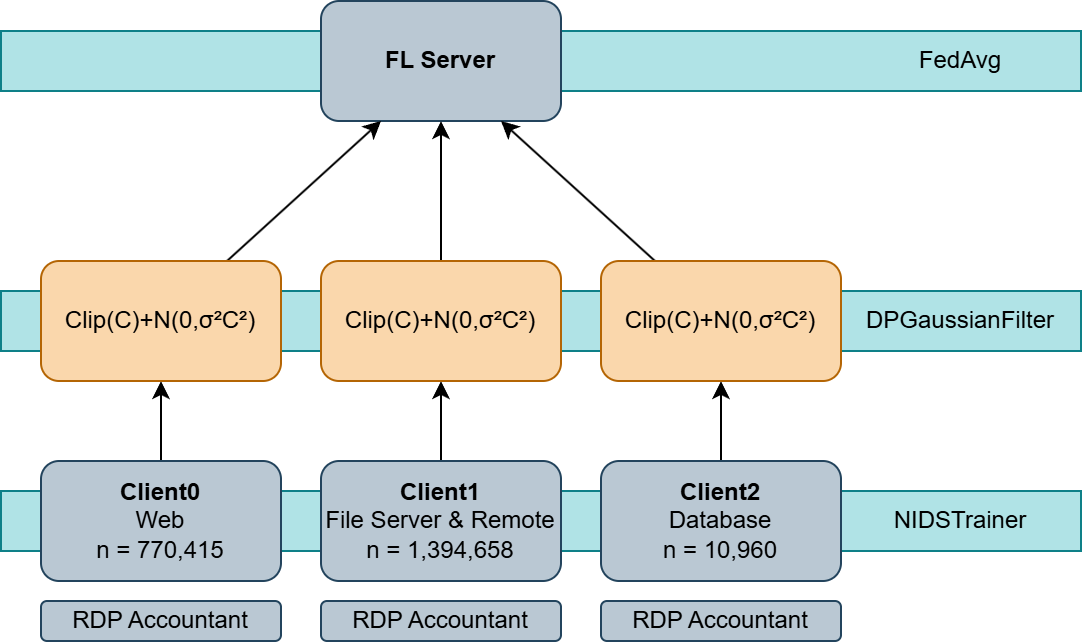
\includegraphics[width=0.99\linewidth]{dp_pipeline}
    \caption{Overview of the Differential Privacy Pipeline.}
    \label{fig:dp_pipeline}
\end{figure}

The DP mechanism was implemented as a custom NVFlare task result filter that intercepts client weight updates after local training and before communication with the federated server. The filter operates directly on the model parameter differences (WEIGHT\_DIFF) generated during local training rounds.

The applied DP pipeline consists of the following stages:
\begin{enumerate}
    \item Flattening the model update tensors into a single vector representation.
    \item Applying L2 norm clipping to bound update sensitivity.
    \item Injecting Gaussian noise proportional to the clipping norm.
    \item Reconstructing the original tensor structure before transmission.
\end{enumerate}

The clipping operation constrains the influence of individual client updates on the global aggregation process, while the Gaussian mechanism introduces randomized perturbations to reduce the risk of information leakage through model inversion or membership inference attacks.

The standard deviation of the injected Gaussian noise is defined as:

$$\sigma_{noise} = \sigma \cdot C$$

where $C$ represents the clipping norm, and $\sigma$ corresponds to the noise multiplier.

Privacy accounting was performed using Rényi Differential Privacy (RDP) composition analysis for the Poisson-subsampled Gaussian mechanism. The privacy accountant tracks the cumulative privacy loss throughout federated training rounds and computes the resulting privacy budget $(\epsilon,\delta)$-DP guarantees for each client individually \cite{mironov2017}.

The sampling rate used in the accounting process is defined as:

$$q=\frac{\text{batch size}}{\text{dataset size}}$$

This formulation is particularly important in heterogeneous federated environments, where clients with smaller datasets accumulate privacy loss more rapidly due to higher sampling probabilities.

The DP hyperparameters are as follows:

\begin{itemize}
    \item Clipping Norm: 2.0
    \item $\delta$: $10^{-5}$
    \item Batch Size: 32
\end{itemize}

% #TODO: change table according to actual runned data

\begin{table}[ht]
    \centering
    \renewcommand{\arraystretch}{1.3}
    \begin{tabular}{|c|c|c|c|c|}
        \hline
        \textbf{Setup} & \textbf{$\sigma$} & \thead{\textbf{Expected $\epsilon$} \\ \textbf{client0}} & \thead{\textbf{Expected $\epsilon$} \\ \textbf{client1}} & \thead{\textbf{Expected $\epsilon$} \\ \textbf{client2}} \\ \hline
        A & 0.37 & 1.1395 & 0.9820 & 9.5548 \\ \hline
        B & 0.30 & 2.1512 & 1.7924 & 18.9338 \\ \hline
        C & 0.25 & 4.1797 & 3.6239 & 41.4177 \\ \hline
        D & 0.24 & 5.5286 & 4.0106 & 54.3336 \\ \hline
        E & 0.23 & 6.4429 & 5.6471 & 75.3987 \\ \hline
        F & 0.22 & 7.8968 & 6.2826 & 111.7086 \\ \hline
        G & 0.21 & 12.5251 & 8.0694 & 178.5184 \\ \hline
        H & 0.20 & 14.4215 & 12.4992 & 311.3686 \\ \hline
    \end{tabular}
    \caption{Privacy Leakage ($\epsilon$) Across Clients by Noise Multiplier}
    \label{tab:dp_client_epsilon}
\end{table}

As seen in \autoref{tab:dp_client_epsilon}, the controlled variable in the experiment is the noice multiplier $\sigma$.

To ensure enforceable privacy guarantees, each client maintains a persistent privacy budget tracker throughout training. Once the cumulative privacy loss exceeds the target privacy budget, the client stops contributing model updates to subsequent federated aggregation rounds.

\section{Results}

\subsection{Centralized Baseline}

The centralized GraphIDS implementation was evaluated to establish a reference point for the subsequent federated learning experiments. The model was trained using the sampled NF-CSE-CIC-IDS2018-v3 subset described in \autoref{subsec:dataset_sampling}.

The centralized configuration achieved a Macro F1-score of 0.9738 and a PR-AUC of 0.8885 on the test dataset. Additionally, the training process required an average of approximately 2.27 seconds per epoch under the experimental hardware configuration described previously.

The obtained results indicate that the GraphIDS architecture is capable of effectively learning graph-based network traffic representations in a centralized environment. The high Macro F1-score demonstrates strong overall classification performance across attack and benign traffic classes, while the PR-AUC result suggests effective discrimination capability under imbalanced traffic conditions.

These results establish the performance baseline against which the FL, SecAgg, and DP configurations are evaluated in the following sections.

\subsection{Federated Learning Performance}

\subsubsection{Global Model Performance}

The federated GraphIDS configuration was evaluated after 100 communication rounds using the FedAvg aggregation strategy described in \autoref{subsec:federated_learning_setup}.

The federated global model achieved a Macro F1-score of 0.9616 and a PR-AUC of 0.8471 on the test dataset. Compared to the centralized baseline, the federated configuration exhibited only a minor reduction in classification performance.

\autoref{tab:performance_comparison_fed} summarizes the comparison between centralized and federated training.

\begin{table}[ht]
    \centering
    \renewcommand{\arraystretch}{1.3}
    \begin{tabular}{|l|c|c|}
        \hline
        \textbf{Configuration} & \textbf{Macro F1} & \textbf{PR-AUC} \\ \hline
        Centralized & 0.9738 & 0.8885 \\ \hline
        Federated & 0.9616 & 0.8471 \\ \hline
    \end{tabular}
    \caption{Performance Comparison between Centralized and Federated Training Configurations}
    \label{tab:performance_comparison_fed}
\end{table}

The observed performance reduction can be attributed to the heterogeneous non-IID distribution of network traffic across clients, where each participant only observes a partial subset of the overall malicious and benign traffic distribution during local training.

\subsubsection{Client Training Dynamics}

\autoref{fig:federated_metrics_clients} presents the evolution of local client metrics throughout federated training, including loss, Macro F1-score, and PR-AUC across communication rounds.

\begin{figure}[ht]
    \centering
    
\includegraphics[width=0.99\linewidth]{metrics_all_clients_2652fb2d-d4fe-45e3-8677-93e2af2b497c}
    \caption{Evolution of federated clients training metrics across communication rounds.}
    \label{fig:federated_metrics_clients}
\end{figure}

The training curves indicate stable convergence behavior across clients despite the heterogeneous traffic distributions introduced by the federated partitioning strategy. Variations between client performance trajectories can be attributed to differences in local dataset size, traffic composition, and class imbalance severity.

Clients containing smaller or more imbalanced datasets exhibited greater metric variability during training, while larger datasets produced more stable convergence patterns.

\subsubsection{Global Model Diagnostic Analysis}

\autoref{fig:federated_global_diagnostic} presents the anomaly score distribution for benign and malicious traffic samples and Precision-Recall (PR) curve obtained from the federated global model.

\begin{figure}[ht]
    \centering
    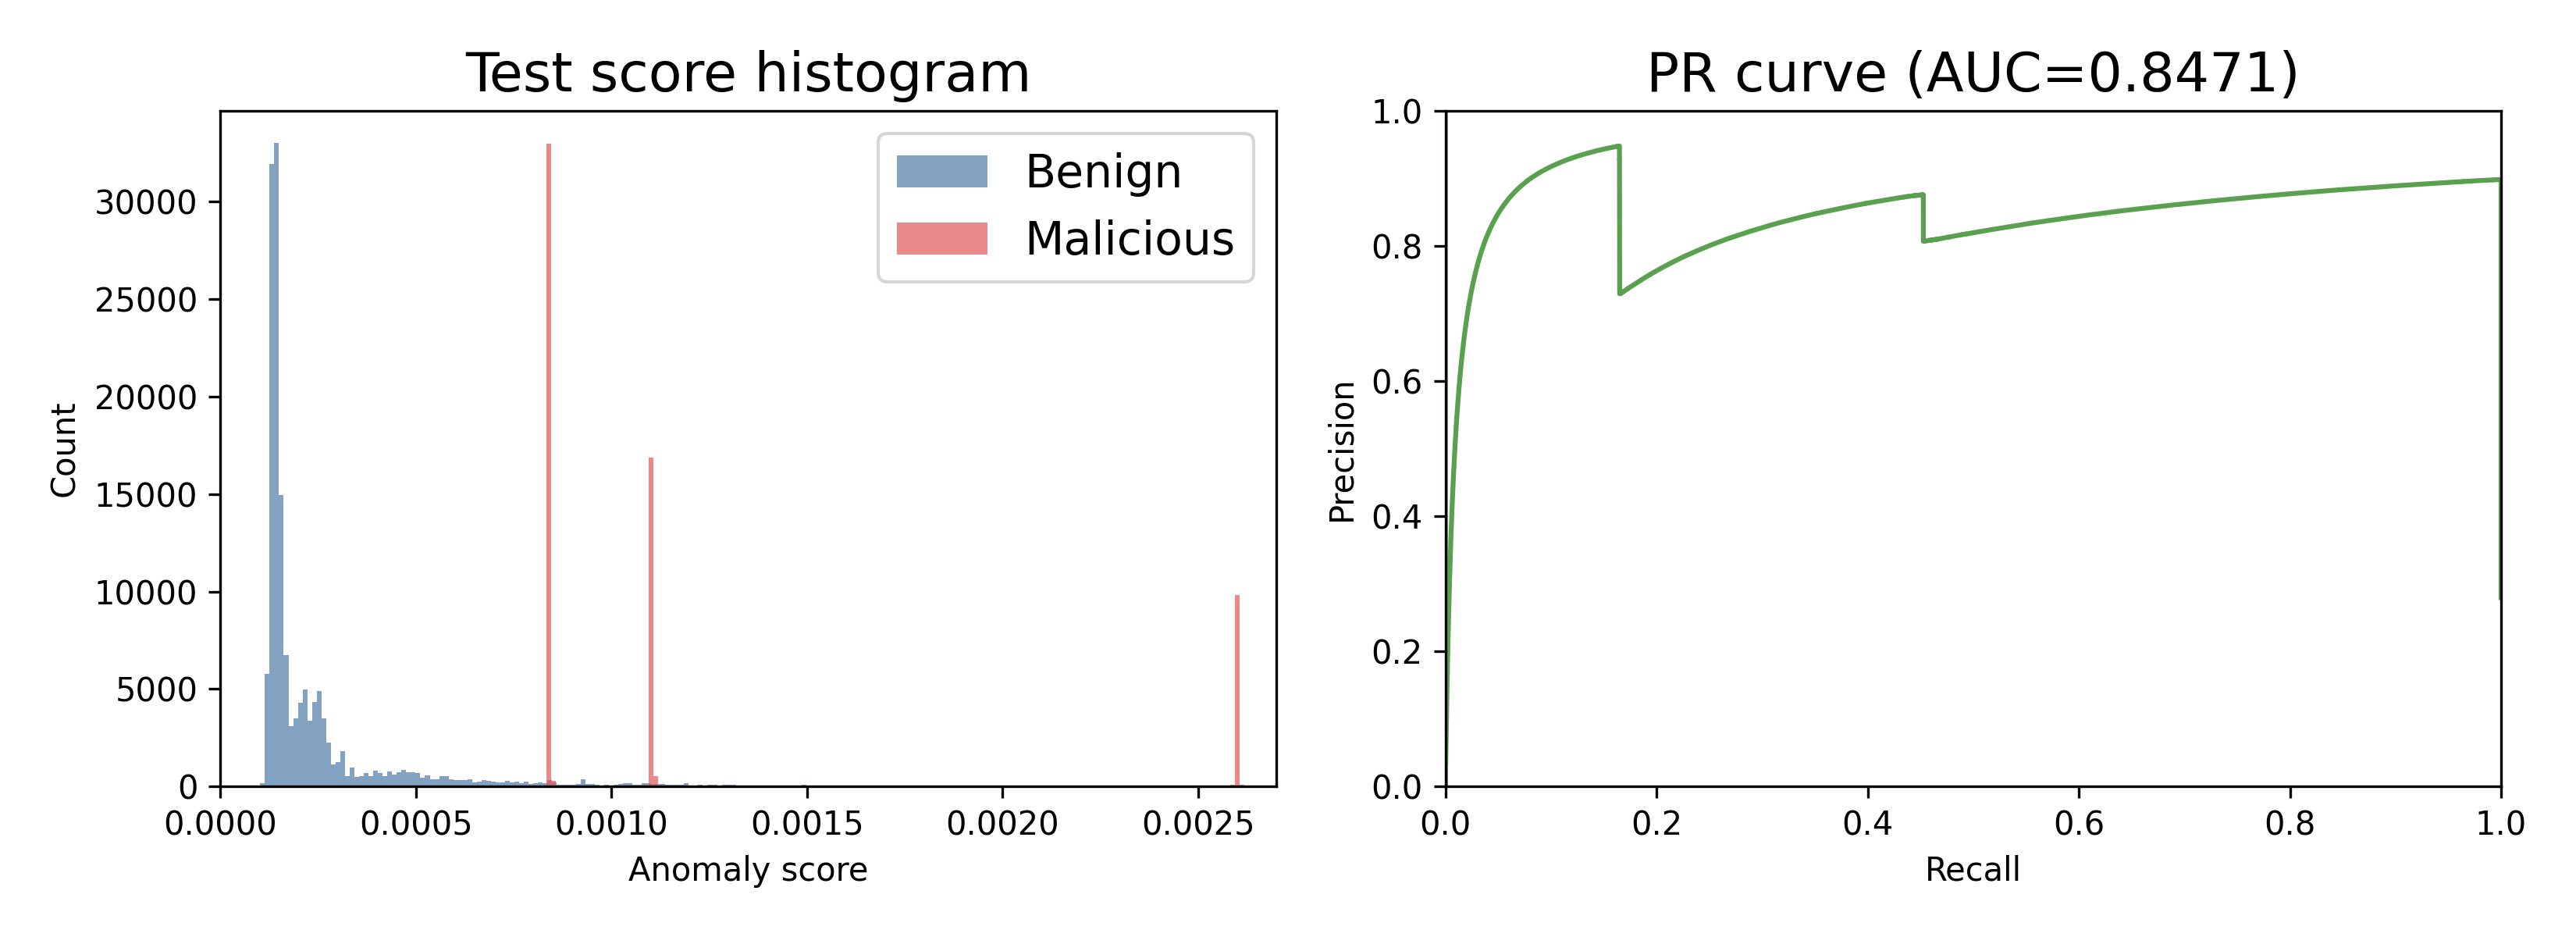
\includegraphics[width=0.99\linewidth]{diagnostics_global_2652fb2d-d4fe-45e3-8677-93e2af2b497c}
    \caption{Anomaly score distribution and Precision-Recall curve of the federated global model.}
    \label{fig:federated_global_diagnostic}
\end{figure}

The PR curve exhibits several localized fluctuations rather than a fully smooth precision transition as recall increases. These variations suggest sensitivity to threshold selection and may be influenced by class imbalance as well as heterogeneous attack distributions across federated clients. Despite these irregularities, the overall curve maintains strong precision-recall behavior consistent with the obtained PR-AUC score.

The anomaly score histogram further demonstrates that the federated model successfully distinguishes malicious traffic from benign network behavior. Most benign samples remain concentrated within lower anomaly score regions, while malicious samples are distributed across higher anomaly score intervals.

Additionally, the histogram reveals multiple concentrated malicious score regions, suggesting that the model captures distinct anomalous traffic patterns associated with different attack behaviors. However, a limited overlap between benign and malicious samples remains visible near lower anomaly score thresholds, indicating the presence of some false positive classifications.

Overall, the diagnostic analysis suggests that the federated GraphIDS model preserves meaningful anomaly discrimination capability despite the heterogeneous and distributed nature of the federated training environment.

\subsubsection{Embedding Space Analysis}

To further analyze the quality of the learned feature representations, t-SNE projections were generated for the embeddings produced by the GNN encoder and for the reconstructed embeddings generated by the Transformer-based reconstruction module.

\autoref{fig:tsne_client0} to \autoref{fig:tsne_client2} present the space visualizations for clients 0, 1, and 2, while Figure \autoref{fig:tsne_fed_baseline} shows the final federated global model representation. These projections provide qualitative insight into the separability between benign and malicious traffic patterns learned during federated training.

\begin{figure}[ht]
    \centering
    
\includegraphics[width=0.99\linewidth]{tSNE_client0}
    \caption{t-SNE projection of client 0 embedding spaces showing separability between benign and malicious traffic for both GNN-generated and Transformer-reconstructed embeddings.}
    \label{fig:tsne_client0}
\end{figure}

As shown in \autoref{fig:tsne_client0}, client 0 exhibits relatively clear separation between benign traffic clusters and anomalous samples. Both the original GNN embeddings and the reconstructed embeddings preserve distinguishable malicious traffic regions within the latent space, indicating that the local model successfully learned representative structural patterns associated with attack behavior.

\begin{figure}[ht]
    \centering
    
\includegraphics[width=0.99\linewidth]{tSNE_client1}
    \caption{t-SNE projection of client 1 embedding spaces illustrating preserved anomaly separation in both original and reconstructed embeddings.}
    \label{fig:tsne_client1}
\end{figure}

A similar behavior can be observed for client 1 in \autoref{fig:tsne_client1}, where malicious samples remain more isolated from the dominant benign traffic clusters. The reconstructed embeddings generated by the Transformer module preserve much of the separability observed in the original GNN representations, suggesting stable reconstruction capability and consistent anomaly representation learning.

\begin{figure}[ht]
    \centering
    
\includegraphics[width=0.99\linewidth]{tSNE_client2}
    \caption{t-SNE projection of client 2 embedding spaces showing reduced separability between benign and malicious traffic embeddings under highly imbalanced local data conditions.}
    \label{fig:tsne_client2}
\end{figure}

In contrast, the representations for client 2 shown in \autoref{fig:tsne_client2} demonstrate significantly reduced separability between benign and malicious traffic samples. Although some anomalous samples occupy slightly displaced regions within the embedding space, the reconstructed malicious representations remain highly overlapped with benign traffic clusters. This reduced space isolation may explain the lower performance observed for client 2 in the training metric analysis presented in the previous subsection.

The reduced representation quality observed in client 2 is likely associated with the severe class imbalance and limited attack diversity present within that federated partition. Under highly imbalanced local traffic distributions, the model receives fewer representative malicious samples during local optimization, limiting its ability to construct well-separated anomalous representations.

\begin{figure*}[ht]
    \centering
    
\includegraphics[width=0.99\linewidth]{tSNE_server_2652fb2d-d4fe-45e3-8677-93e2af2b497c}
    \caption{t-SNE projection of the federated global model embedding spaces demonstrating generalized anomaly representation learned across heterogeneous clients.}
    \label{fig:tsne_fed_baseline}
\end{figure*}

Despite the variability observed across local clients, the final federated global model shown in \autoref{fig:tsne_fed_baseline} preserves meaningful cluster structure and maintains distinguishable anomalous regions within the shared latent space. These observations suggest that the federated aggregation process successfully captures generalized traffic behavior patterns while combining heterogeneous representations learned across distributed clients.

\subsubsection{Computational and Communication Cost}

The federated learning configuration introduced additional computational and communication overhead compared to the centralized baseline due to distributed training coordination, repeated model synchronization, and parameter aggregation operations.

The centralized GraphIDS implementation required approximately 2.27 seconds per training epoch, while the federated configuration completed 100 communication rounds in approximately 43 minutes and 54 seconds. Considering that each client performed two local epochs per round, the federated setup executed approximately 200 local training epochs per client during the experiment.

Although the effective local epoch duration in the federated setting was moderately higher than the centralized configuration, this increase does not solely reflect local model training cost. Additional overhead is introduced by federated communication, parameter serialization, synchronization barriers, and FedAvg aggregation performed during each communication round.

From the server perspective, the federated training process exchanged approximately 1.29 GB of model data throughout training. The server transmitted approximately 660.52 MB to clients and received approximately 660.70 MB of client updates. Each federated client exchanged approximately 440 MB of model parameters during the experiment.

\autoref{tab:comm_metrics_fed_baseline} summarizes the communication statistics observed during federated training.

\begin{table}[ht]
    \centering
    \renewcommand{\arraystretch}{1.3}
    \begin{tabular}{|l|c|}
        \hline
        \textbf{Metric} & \textbf{Value} \\ \hline
        Total Communication Volume & 1.29 GB \\ \hline
        Total Sent to Clients & 660.52 MB \\ \hline
        Total Received from Clients & 660.70 MB \\ \hline
        Per-Client Communication & $\sim$440 MB \\ \hline
        Communication Rounds & 100 \\ \hline
        Training Time & 43m 54s \\ \hline
    \end{tabular}
    \caption{Federated Learning Communication Cost and Execution Runtime}
    \label{tab:comm_metrics_fed_baseline}
\end{table}

These results demonstrate that federated learning preserves intrusion detection capability with relatively moderate communication overhead under the evaluated experimental configuration. However, the observed communication cost also highlights one of the primary scalability challenges associated with federated learning systems, particularly when privacy-preserving mechanisms such as SecAgg and DP are incorporated into the training pipeline.

\subsection{Impact of Secure Aggregation}

This section evaluates the impact of HE-based SecAgg on federated intrusion detection performance, computational cost, and communication overhead.

The SecAgg pipeline was integrated using the CKKS-HE scheme described in \autoref{subsec:secure_aggregation}. Under this configuration, client model updates were encrypted locally before transmission, preventing the aggregation server from accessing plaintext model parameters during Federated Averaging.

The evaluation focuses on the trade-off between confidentiality preservation and system efficiency by comparing the standard federated learning configuration against the encrypted aggregation pipeline.

\autoref{tab:secagg_comparison} summarizes the overall impact of HE-based SecAgg on federated intrusion detection performance, runtime, and communication overhead.

\begin{table}[ht]
    \centering
    \renewcommand{\arraystretch}{1.3}
    \begin{tabular}{|l|c|c|c|c|}
        \hline
        \textbf{Configuration} & \thead{\textbf{Macro}\\\textbf{F1}} & \thead{\textbf{PR-}\\\textbf{AUC}} & \textbf{Runtime} & \thead{\textbf{Total}\\\textbf{Comm.}} \\ \hline
        Federated & 0.9616 & 0.8471 & 43m 54s & 1.29 GB \\ \hline
        Federated + SecAgg & 0.8968 & 0.7479 & 1h 17m 43s & 31.99 GB \\ \hline
    \end{tabular}
    \caption{Performance, Execution Runtime, and Overhead Metrics under Secure Aggregation}
    \label{tab:secagg_comparison}
\end{table}

The SecAgg configuration introduced measurable performance degradation together with substantial computational and communication overhead. Nevertheless, the encrypted federated pipeline maintained effective intrusion detection capability while preventing the aggregation server from accessing plaintext client updates.

\subsubsection{Performance Comparison}

The integration of homomorphic encryption-based secure aggregation introduced a measurable reduction in intrusion detection performance compared to the standard federated learning configuration.

As shown in \autoref{tab:secagg_comparison}, the secure aggregation pipeline achieved a Macro F1-score of 0.8968 and a PR-AUC of 0.7479, compared to 0.9616 and 0.8471 obtained under the plaintext federated setting. Despite this degradation, the encrypted federated model preserved effective anomaly detection capability across the evaluated traffic distributions.

The observed performance reduction may be associated with the numerical approximation behavior of the CKKS-HE scheme, together with the additional instability introduced by encrypted aggregation operations during federated optimization. Nevertheless, the resulting model maintained strong classification capability while preventing the aggregation server from accessing plaintext client updates.

\subsubsection{Computational Overhead}

SeccAgg significantly increased the computational cost of federated training. The encrypted configuration required approximately 1 hour and 17 minutes to complete training, compared to 43 minutes for the standard federated learning pipeline.

The additional runtime overhead originates primarily from homomorphic encryption operations performed during client-side parameter encryption, encrypted aggregation at the server, and ciphertext decryption during synchronization rounds. Compared to plaintext aggregation, these cryptographic operations introduce substantially higher computational complexity during each federated communication cycle.

Despite the increased runtime, the encrypted training process remained stable throughout all communication rounds, demonstrating the feasibility of integrating homomorphic encryption into federated intrusion detection environments.

\subsubsection{Communication Overhead}

The largest overhead introduced by secure aggregation was observed in communication cost. The encrypted federated configuration exchanged approximately 31.99 GB of model data during training, compared to 1.29 GB in the plaintext federated setting.

This increase is primarily associated with ciphertext expansion produced by the CKKS homomorphic encryption scheme. Encrypted model parameters require significantly larger serialized representations than plaintext tensors, resulting in substantially higher transmission volume during each federated round.

The observed communication overhead highlights one of the primary scalability challenges of homomorphic encryption-based federated learning systems, particularly in bandwidth-constrained or large-scale distributed environments.

\subsubsection{Training Stability}

\begin{figure}[ht]
    \centering
    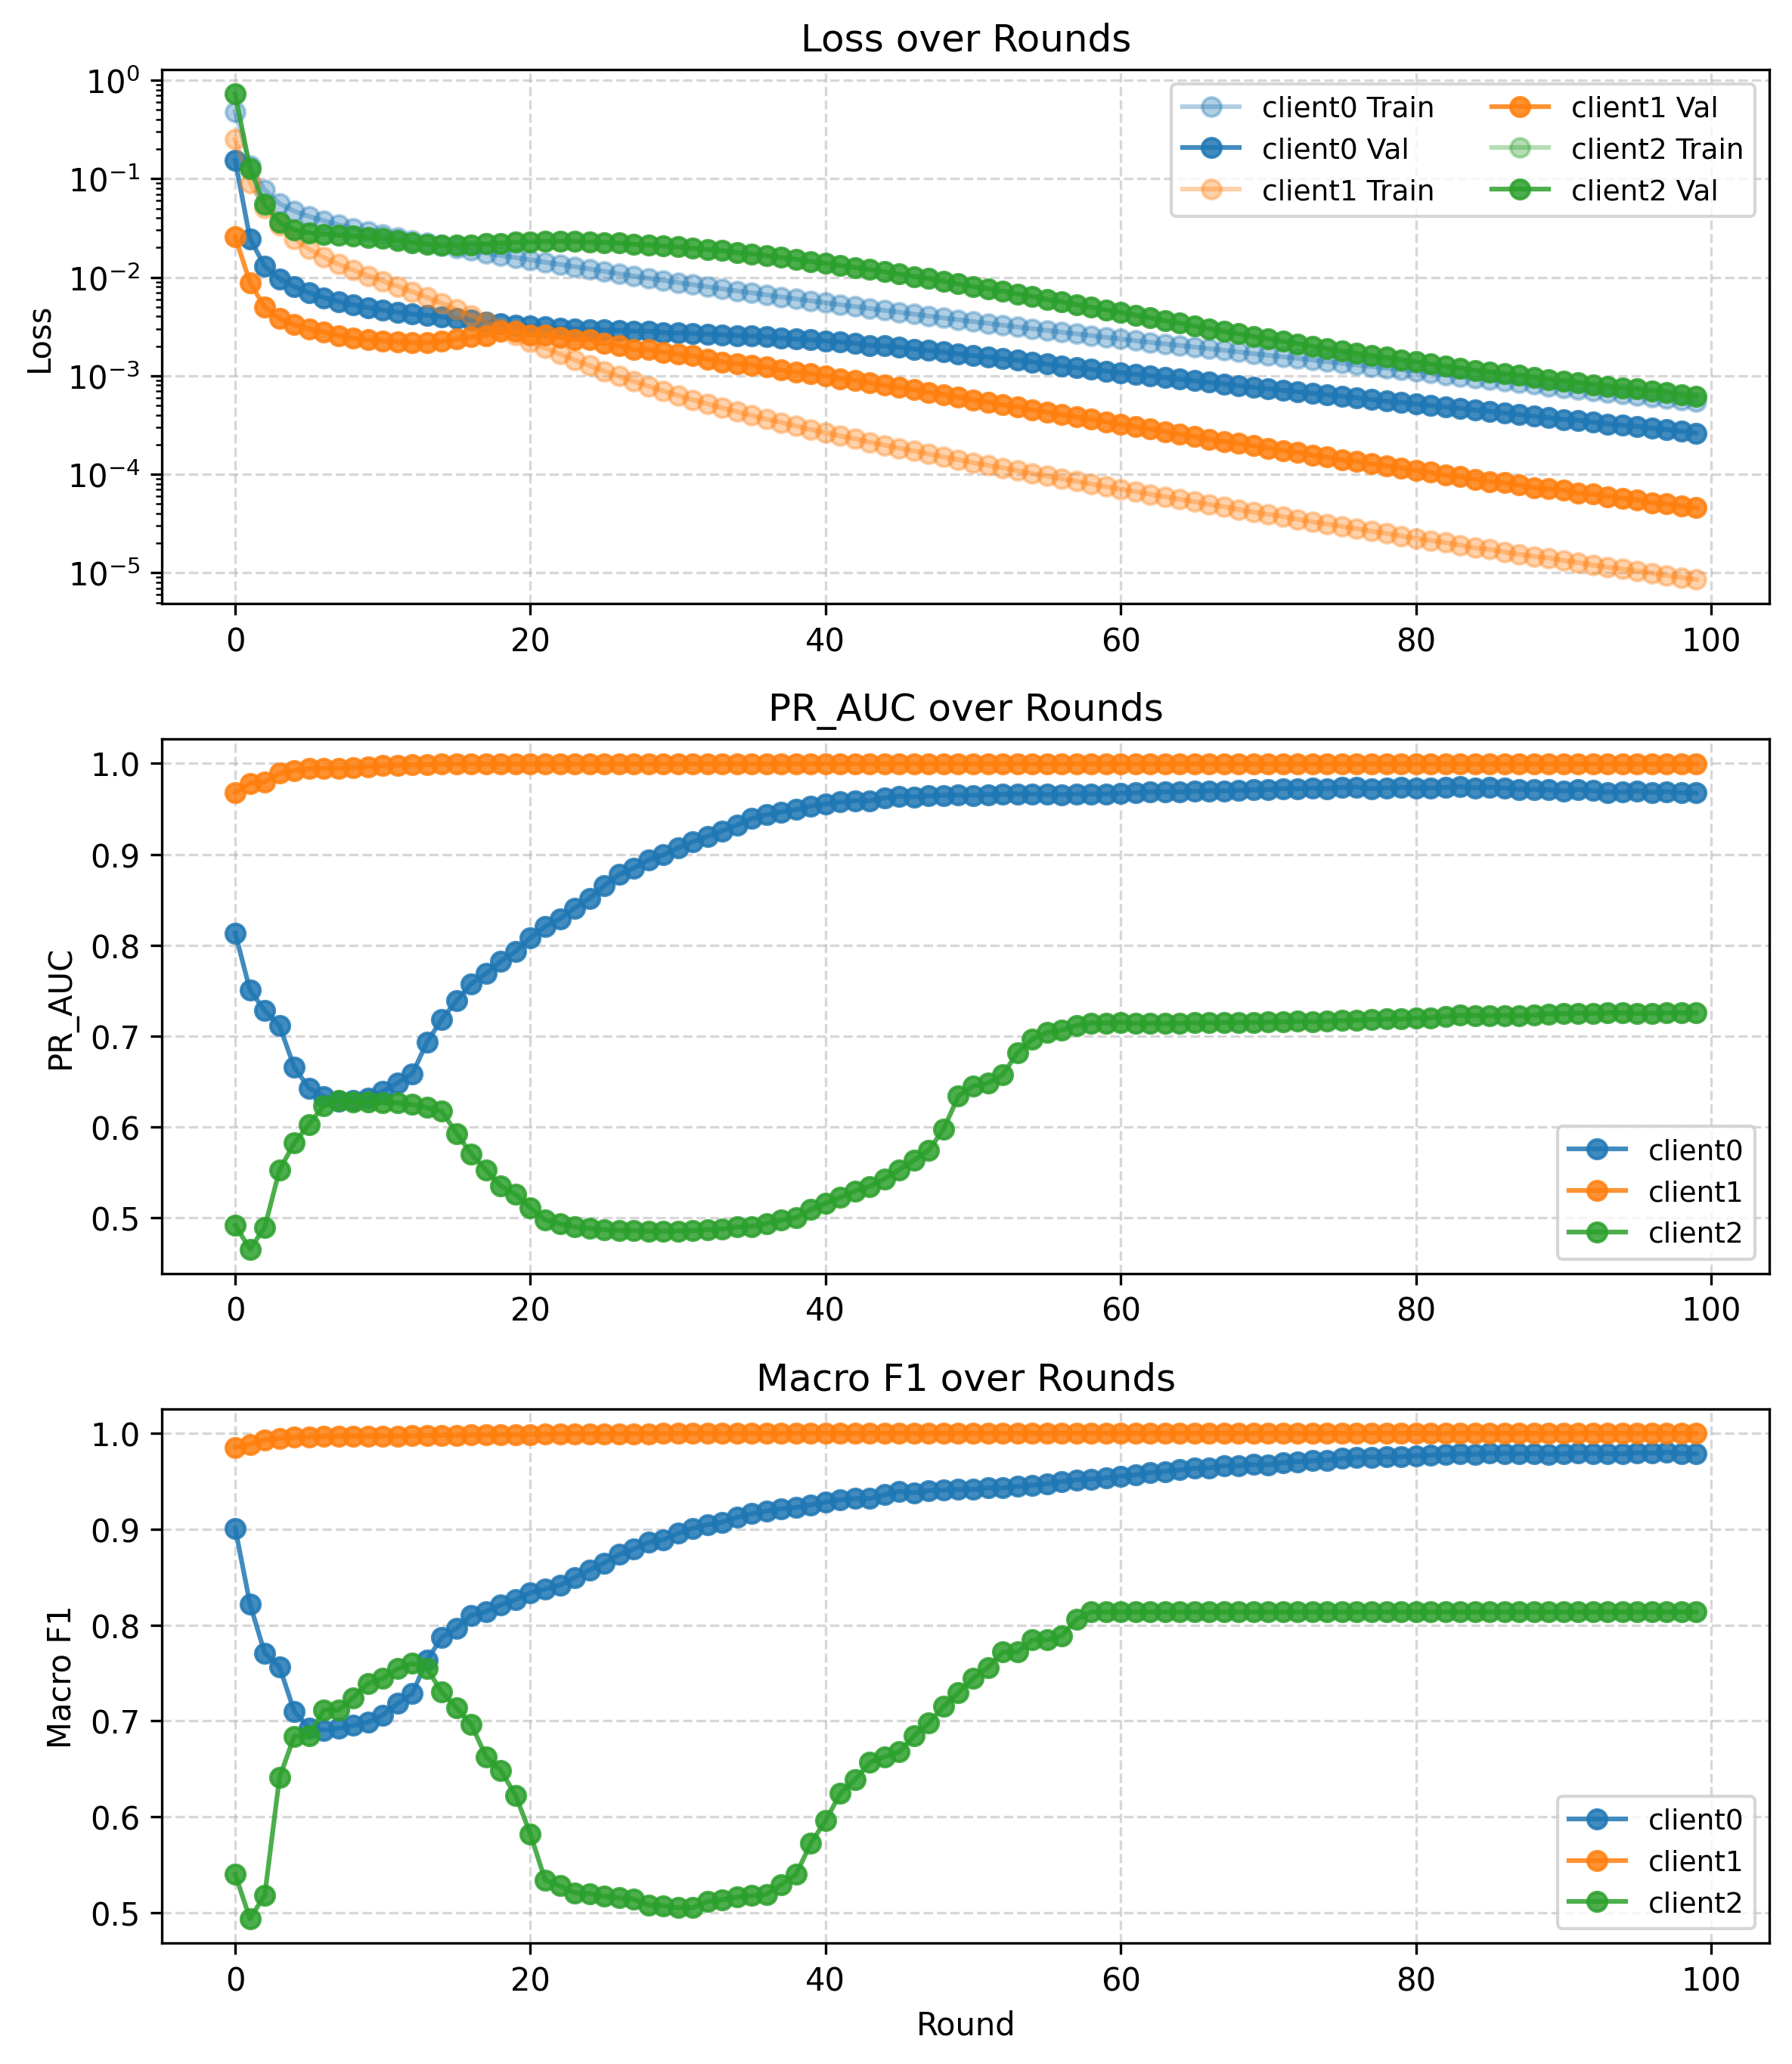
\includegraphics[width=0.99\linewidth]{metrics_all_clients_48ade0c8-a00c-4591-bccb-7803945a0aa4}
    \caption{Evolution of federated clients with SecAgg training metrics across communication rounds.}
    \label{fig:federated_metrics_clients_seccagg}
\end{figure}

\autoref{fig:federated_metrics_clients_seccagg} presents the evolution of training loss, Macro F1-score, and PR-AUC throughout the SecAgg training process for each federated client.

The loss curves exhibit consistent downward trends across all clients, indicating that the encrypted federated optimization process remained capable of learning meaningful traffic representations despite the additional cryptographic operations introduced during aggregation.

The evaluation metrics, however, display greater variability across communication rounds compared to the plaintext federated configuration. Client 0 initially experienced a reduction in PR-AUC performance before progressively recovering and converging toward higher values during later training rounds. A similar trend was observed for the Macro F1-score, suggesting temporary fluctuations in local model generalization during intermediate aggregation stages.

Client 2 exhibited the highest degree of metric variability and remained the lowest-performing participant throughout training. Both PR-AUC and Macro F1-score initially improved during early communication rounds, followed by intermediate performance degradation and subsequent recovery during later stages of training. This behavior is consistent with the heterogeneous and highly imbalanced data distribution assigned to this client, which likely increases optimization sensitivity under encrypted federated aggregation.

Despite the observed oscillatory behavior in evaluation metrics, the training process did not exhibit optimization collapse or divergence. Instead, all clients ultimately demonstrated convergence toward stable performance regions, indicating that HE-based SecAgg preserves the feasibility of collaborative federated intrusion detection training, although with reduced optimization stability compared to plaintext FL.

\subsubsection{Security Implications}

The SeccAgg configuration significantly improves the confidentiality of the federated training process by preventing the aggregation server from accessing plaintext client model updates during training.

Under the implemented CKKS-HE pipeline, model parameters are encrypted locally at each client before transmission. The aggregation server performs FedAvg directly over encrypted ciphertexts without decrypting the underlying model weights. As a result, raw client updates remain inaccessible throughout the aggregation process.

This design reduces the risk of sensitive information exposure through direct inspection of client model parameters and mitigates potential leakage associated with centralized access to local training updates. Such protections are particularly relevant in intrusion detection environments, where model updates may implicitly contain information related to internal network behavior, traffic patterns, or attack activity.

However, the experimental results also demonstrate that these confidentiality improvements introduce substantial computational and communication overhead. Consequently, HE-based SecAgg represents a trade-off between privacy preservation and system efficiency within federated intrusion detection systems.

\subsection{Impact of Differential Privacy}

\subsubsection{Privacy-Utility Tradeoff Overview}

% #TODO: Hacer tabla X!!!

Table X summarizes the impact of different Differential Privacy noise multiplier configurations on federated intrusion detection performance and resulting privacy guarantees.

% #TODO: Hacer grafica de la tabla!!!

Figure X further illustrates the relationship between the noise multiplier, model utility, and cumulative privacy budget.

The evaluated Differential Privacy configurations introduced substantial degradation in intrusion detection performance compared to the plaintext federated learning baseline. Although increasing the noise multiplier reduced the cumulative privacy budget ($\epsilon$), the resulting privacy guarantees remained excessively large across all evaluated configurations.

The best-performing configuration under the evaluated settings was obtained with a noise multiplier of 0.18, achieving a Macro F1-score of 0.7557 and a PR-AUC of 0.4388. However, even under this configuration, the cumulative privacy loss remained significantly above values typically considered practical for strong DP guarantees.

These results suggest that the evaluated client-side Gaussian perturbation mechanism produces a difficult privacy-utility trade-off within the GraphIDS federated learning architecture. Under the tested heterogeneous and non-IID federated environment, increasing privacy protection resulted in substantial reductions in model stability and intrusion detection capability while still failing to achieve practically useful privacy budgets.

\subsubsection{Privacy Budget Progression}

% #TODO

\subsubsection{Training Stability}

% #TODO

\subsubsection{Impact of Noise Multiplier}

% #TODO

\subsubsection{Practical Limitations}

% #TODO

\section{Discussion}



\section{Conclusion}



\section*{Acknowledgment}

The author thanks the Universidad de los Andes for  all the academic support provided. The author also thanks all teachers, especially Ph.D. Yuri Andrea Pinto as this thesis advisor.

The authors would like to acknowledge the use of LLMs to assist in grammatical refinement, copyediting, and text redaction during the preparation of this manuscript. All primary content, technical claims, and experimental interpretations remain the sole responsibility of the authors.

\bibliographystyle{IEEEtran}
\bibliography{references}

\end{document}